\documentclass[17pt]{extarticle}
\usepackage{tikz}
\usepackage{showexpl}
\usepackage{gensymb}
\usetikzlibrary{arrows.meta}
\usepackage[top=0.2in,left=0.9in,right=1cm]{geometry} %This geometry is page layout

\usepackage{titlesec}
%%%%%%%%%%%%%%%%
% For Title  content index
%\usepackage[utf8]{inputenc}
%\title{Latex Diagram Referrence}
%\author{ILUG-BOM}
%\date{ }
%%%%%%%%%%%%%%%%%%
\lstset
{   language=[LaTeX]TeX,
    breaklines=true,
    basicstyle=\fontsize{14}{14}\ttfamily,
    keywordstyle=\color{blue},
    identifierstyle=\color{magenta},
}

\begin{document}

\titleformat{\section}{\normalfont\normalsize\bfseries}{\thesection}{1em}{}
\titlespacing{\section}{0pt}{0pt}{-0.3 cm}  

%%%%%%%%%%%%%%%%%%%%%%%%%%%%%%%%%%
%\maketitle
%\tableofcontents
%\clearpage

%%%%%%%%%%%%%%%%%%%%%%%%%%%%%%%%%%%%%%%%%%%%%%%
%%%%%%%%%%%%%%%%%%%%%%%%%%%%%%%%%%%%%%%%%
%%%%%%%%%%%%%%%%%%%%%%%%%%%%%%%%%%%%%%%%%Start Examples
%%%%%%%%%%%%%%%%%%%%%%%%%%%%%%%%%%%%%%%%%
%%%%%%%%%%%%%%%%%%%%%%%%%%%%%%%%%%%%%%%%%

\section {Background Grid}

\begin{LTXexample}[pos=b,preset=\centering,width=1\linewidth]
  
\begin{tikzpicture}
  
    \draw[very thin, gray!30, step=1 cm](-5,-5) grid (5,5);
  
  \end{tikzpicture}
\end{LTXexample}

\pagebreak

%%%%%%%%%%%%%%%%%%%%%%%%%%%%%%%%%%%%%%%%%%%%%%%%%%%%%%%%%%%%

\section {Angle}

\begin{LTXexample}[pos=b,preset=\centering,width=1\linewidth]
  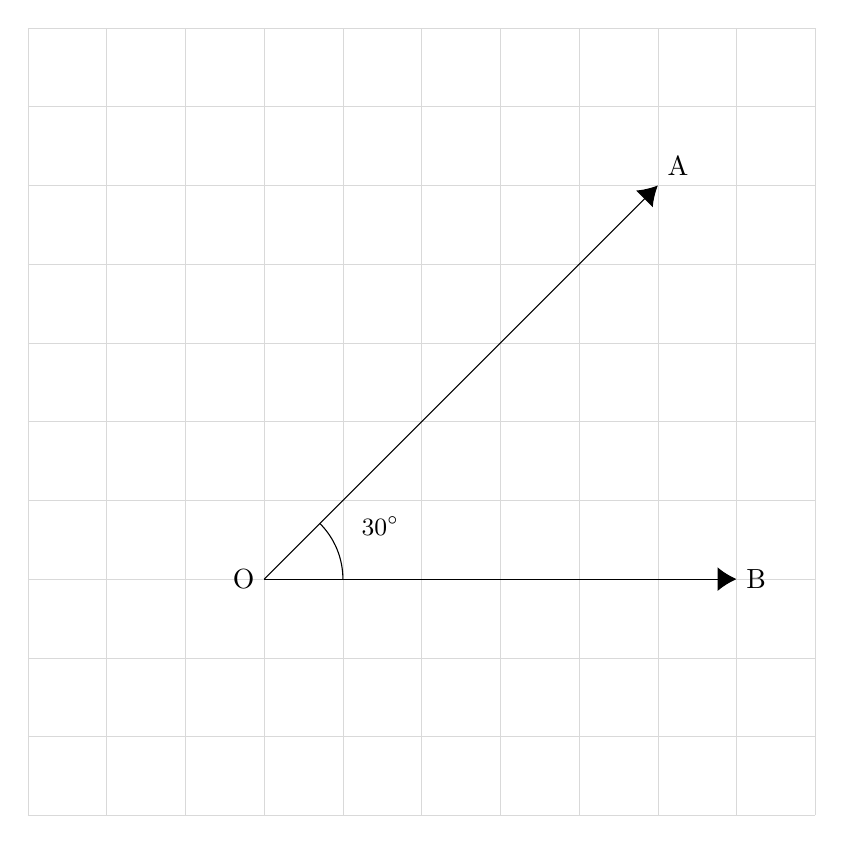
\begin{tikzpicture}
   \draw[very thin, gray!30, step=1 cm](0,0) grid (10,10);
   \draw [>={LaTeX[width=3mm,length=2.4mm]},->](3,3) node[left]{O}--(8,8) node[above right]{A}; 
   \draw [>={LaTeX[width=3mm,length=2.4mm]},->](3,3)--(9,3) node[right]{B}; 
    \draw (4,3) arc (0:45:1cm);
    \draw (3,3) node[anchor=north, xshift=42pt, yshift=26pt, font=\small] {$30\degree$};
  \end{tikzpicture}
\end{LTXexample}

\pagebreak

%%%%%%%%%%%%%%%%%%%%%%%%%%%%%%%%%%%%%%%%%%%%%%%
\section {Angle - Slope Naming and Font Change}

\begin{LTXexample}[pos=b,preset=\centering,width=1\linewidth]
  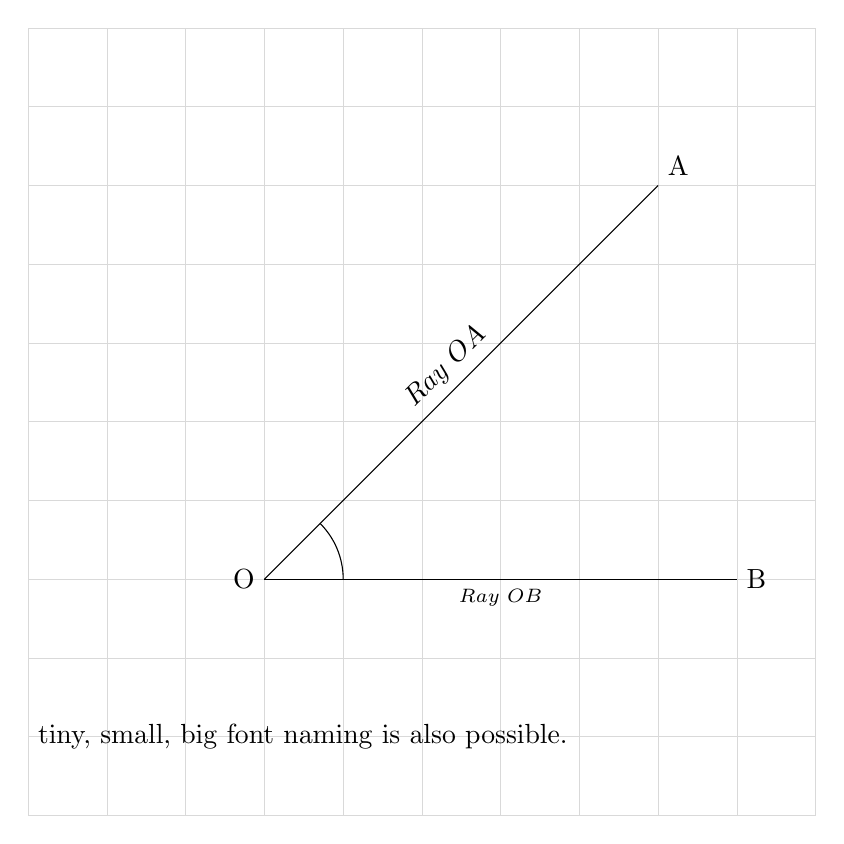
\begin{tikzpicture}
   \draw[very thin, gray!30, step=1 cm](0,0) grid (10,10);
   \draw (3,3) node[left]{O}-- node[above,sloped]{$Ray\,\,OA$}(8,8) node[above right]{A}; 
   \draw (3,3)--node[below,sloped]{\scriptsize $Ray\,\,OB$}(9,3) node[right]{B}; 
    \draw (4,3) arc (0:45:1cm);
   \draw (0,1)--(0,1)  node[right]{tiny, small, big font naming is also  possible.};
  \end{tikzpicture}
\end{LTXexample}

\pagebreak

%%%%%%%%%%%%%%%%%%%%%%%%%%%%%%%%%%%%%%%%%%%%%%%
\section {Cartesian Coordinate System - Mid Origin}

\begin{LTXexample}[pos=b,preset=\centering,width=1\linewidth]
  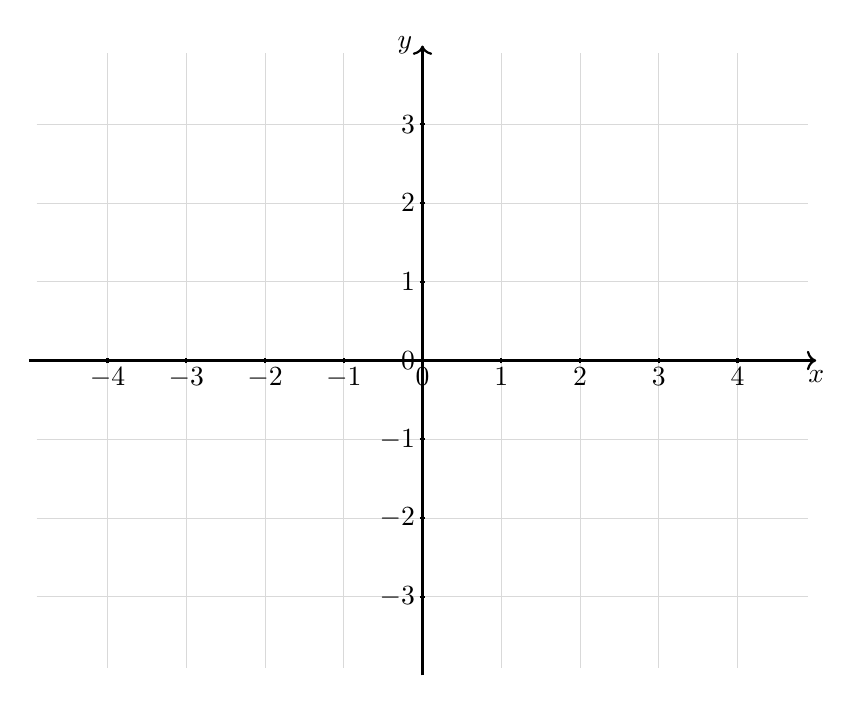
\begin{tikzpicture}
    \draw[very thin, gray!30, step=1 cm](-4.9,-3.9) grid (4.9,3.9);
    \draw [thick] [->] (-5,0)--(5,0) node[right, below] {$x$};
     \foreach \x in {-4,...,4}
       \draw[xshift=\x cm, thick] (0pt,-1pt)--(0pt,1pt) node[below] {$\x$};
      \draw [thick] [->] (0,-4)--(0,4) node[above, left] {$y$};
     \foreach \y in {-3,...,3}
       \draw[yshift=\y cm, thick] (-1pt,0pt)--(1pt,0pt) node[left] {$\y$};
   
  \end{tikzpicture}
\end{LTXexample}

\pagebreak

%%%%%%%%%%%%%%%%%%%%%%%%%%%%%%%%%%%%%%%%%%%%%%%%%%%%%%%%
\section {Cartesian Coordinate System - Bot Left Origin}

\begin{LTXexample}[pos=b,preset=\centering,width=1\linewidth]
  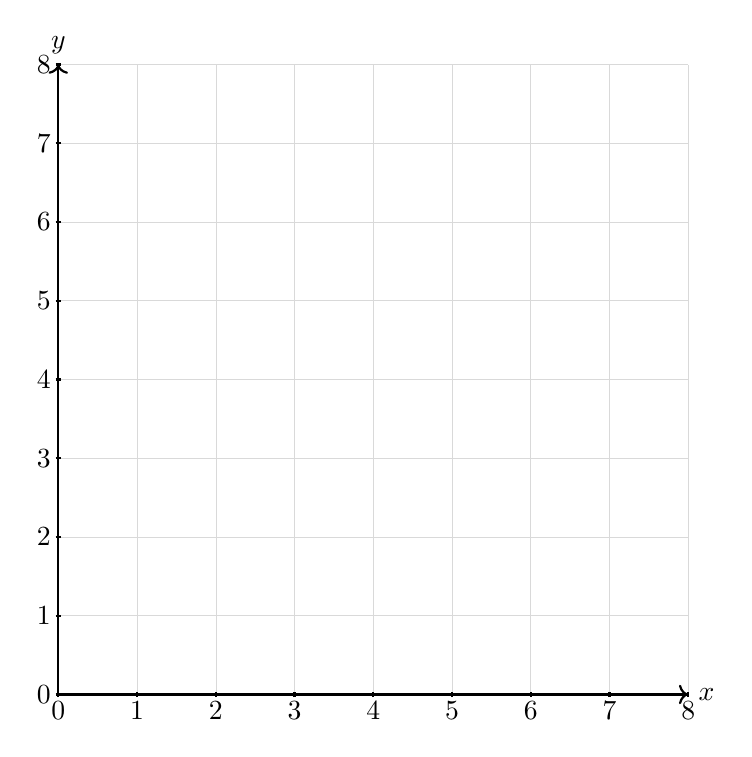
\begin{tikzpicture}
    \draw[very thin, gray!30, step=1 cm](0,0) grid (8,8);
    \draw [thick] [->] (0,0)--(8,0) node[right] {$x$};
     \foreach \x in {0,...,8}
       \draw[xshift=\x cm, thick] (0pt,-1pt)--(0pt,1pt) node[below] {$\x$};
      \draw [thick] [->] (0,0)--(0,8) node[above] {$y$};
     \foreach \y in {0,...,8}
       \draw[yshift=\y cm, thick] (-1pt,0pt)--(1pt,0pt) node[left] {$\y$};
   
  \end{tikzpicture}
\end{LTXexample}

\pagebreak

%%%%%%%%%%%%%%%%%%%%%%%%%%%%%%%%%%%%%%%%%%%%%%%%%%%%%%%%


\section {Pair Of Straight Lines}

\begin{lstlisting}
=====================
Requires :
{\usepackage{gensymb}
\usetikzlibrary{arrows.meta}
==============
\end{lstlisting}


\begin{LTXexample}[pos=b,preset=\centering,width=1\linewidth]
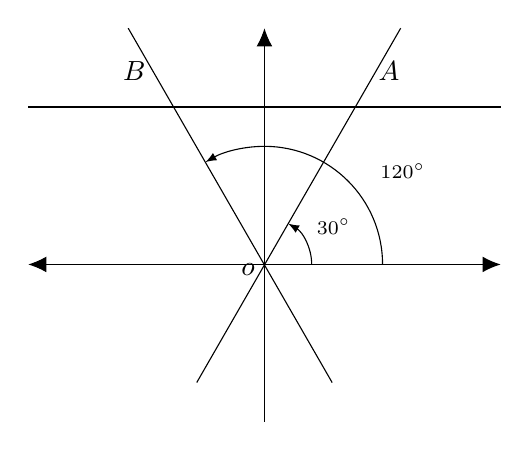
\begin{tikzpicture}
\draw [>={LaTeX[width=2mm,length=2.3mm]},<->](-3,0) -- (3,0); %% X-AXIS
\draw [>={LaTeX[width=2mm,length=2.3mm]},->](0,-2)  -- (0,3); %% Y-AXIS
\draw (-3,2) -- (3,2);
\draw (-0.86,-1.5) -- (1.73,3);
\draw (-1.73,3) -- (0.86,-1.5);
\draw (0,0) node[anchor=north east,yshift=4pt] {$o$} ;
\draw (0,0) node[anchor=north, xshift=45pt, yshift=77pt] {$A$} ;
\draw (0,0) node[anchor=north, xshift=-47pt, yshift=77pt] {$B$}; 
\draw (0,0) node[anchor=north, xshift=50pt, yshift=40pt, font=\scriptsize] {$120\degree$};
\draw (0,0) node[anchor=north, xshift=25pt, yshift=20pt, font=\scriptsize] {$30\degree$};
\draw[-latex] (0:0.6cm) arc (0:60:0.6cm);
\draw[-latex] (0:1.5cm) arc (0:120:1.5cm);
\end{tikzpicture}

\end{LTXexample}
\pagebreak

%%%%%%%%%%%%%%%%%%%%%%%%%%%%%%%%%%%%%%%%%%%%%%%%%%%%%
\section {Cube - Unfolded}
\begin{LTXexample}[pos=b,preset=\centering,width=1\linewidth]
\vspace*{4mm} %to keep box edge little away
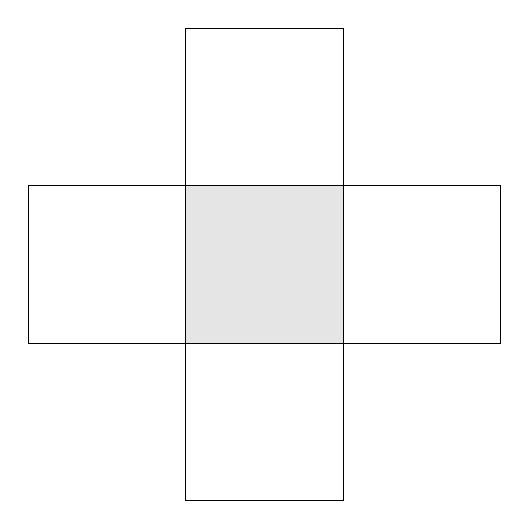
\begin{tikzpicture}
\draw (0,0) -- (0,2) -- (2,2) -- (2,4) -- (4,4) -- (4,2) -- (6,2) -- (6,0) -- (4,0) -- (4,-2) -- (2,-2) -- (2,0) -- (0,0) ; 
\filldraw[fill=gray!20] (2,0) rectangle (4,2);
\end{tikzpicture}
\vspace*{4mm} %to keep box edge little away
\end{LTXexample}
\pagebreak


\section {Cone}
\begin{LTXexample}[pos=b,preset=\centering,width=1\linewidth]
\vspace*{4mm} %to keep box edge little away
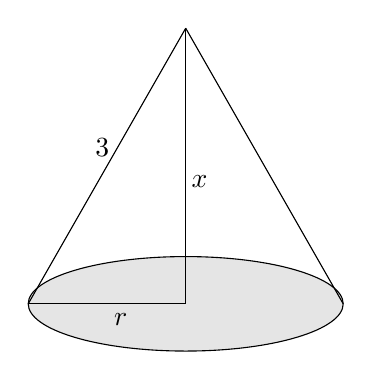
\begin{tikzpicture}
\filldraw[fill=gray!20](0,0) ellipse (2cm and 0.6cm);
\draw (0,0) -- node[below] {\ \ \ $x$}(0,3.5);
\draw (0,0)  -- node[below] {\ \ \ $r$} (-2,0);
\draw  (-2,0) --node[above] {3\ \ }(0,3.5);
\draw  (2,0) -- (0,3.5);
\end{tikzpicture}
\vspace*{4mm} %to keep box edge little away
\end{LTXexample}
\pagebreak
%%%%%%%%%%%%%%%%%%%%%%%%%%%%%%%%%%%%%%%
\section {Cartesian Coordinate System - 1}

\begin{LTXexample}[pos=b,preset=\centering,width=1\linewidth]
  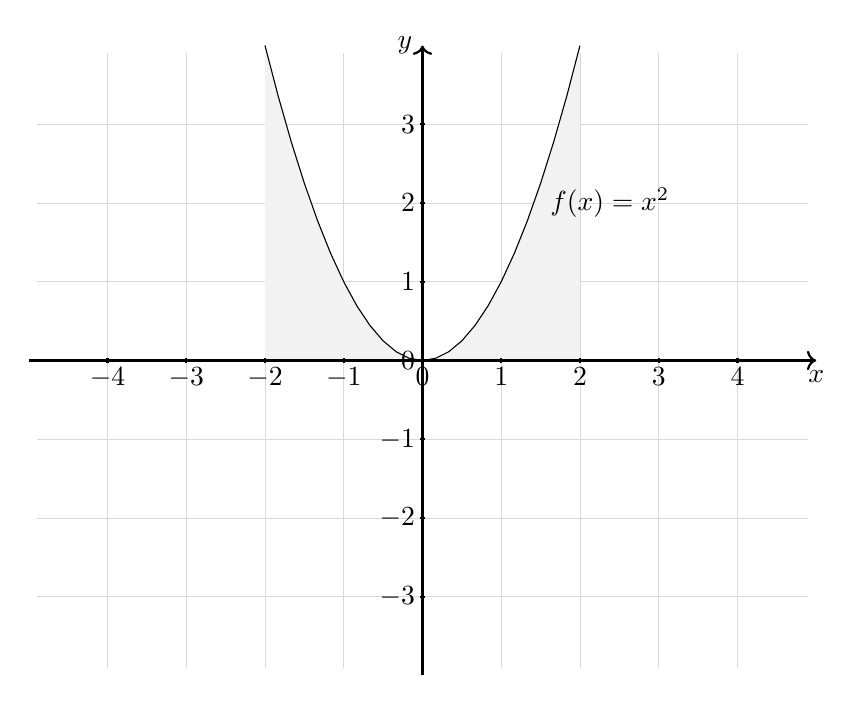
\begin{tikzpicture}
    \draw[very thin, gray!30, step=1 cm](-4.9,-3.9) grid (4.9,3.9);
    \fill [gray!10, domain=-2:2, variable=\x]
     (-2, 0) -- plot ({\x}, {\x*\x}) -- (2, 0) -- cycle;
    \draw [thick] [->] (-5,0)--(5,0) node[right, below] {$x$};
     \foreach \x in {-4,...,4}
       \draw[xshift=\x cm, thick] (0pt,-1pt)--(0pt,1pt) node[below] {$\x$};
      \draw [thick] [->] (0,-4)--(0,4) node[above, left] {$y$};
     \foreach \y in {-3,...,3}
       \draw[yshift=\y cm, thick] (-1pt,0pt)--(1pt,0pt) node[left] {$\y$};

    \draw [domain=-2:2, variable=\x]
      plot ({\x}, {\x*\x}) node[right] at (1.5,2) {$f(x)=x^2$};
  \end{tikzpicture}
\end{LTXexample}

\pagebreak

%%%%%%%%%%%%%%%%%%%%%%%%%%%%%%%%%%%%%%%%%%%%%%%%%%%%%%%%



\end{document}
